% IEEE conference paper with TikZ diagrams for Edge & Cloud Computing review
\documentclass[conference]{IEEEtran}
\IEEEoverridecommandlockouts

% Packages
\usepackage[utf8]{inputenc}
\usepackage[T1]{fontenc}
\usepackage{lmodern}
\usepackage{amsmath,amssymb}
\usepackage{graphicx}
\usepackage{booktabs}
\usepackage{array}
\usepackage{xcolor}
\usepackage{hyperref}
\usepackage{siunitx}
\usepackage{subcaption}
\usepackage{cite}
\usepackage{tikz}
\usetikzlibrary{arrows.meta,positioning,fit,shapes,calc,backgrounds}

% Colors
\definecolor{cloudblue}{HTML}{1F77B4}
\definecolor{edgeteal}{HTML}{17BECF}
\definecolor{fogpurple}{HTML}{9467BD}
\definecolor{latencyred}{HTML}{D62728}
\definecolor{energygreen}{HTML}{2CA02C}
\definecolor{neutralgray}{HTML}{7F7F7F}
\definecolor{gold}{HTML}{BCBD22}
\definecolor{orange}{HTML}{FF7F0E}

% Hyperref setup
\hypersetup{
  colorlinks=true,
  linkcolor=cloudblue,
  citecolor=cloudblue,
  urlcolor=cloudblue
}

\title{EDGE \& CLOUD COMPUTING: A REVIEW OF ARCHITECTURE, CHALLENGES, AND FUTURE DIRECTIONS}

% NOTE: Replace with real authors and affiliations prior to submission
\author{\IEEEauthorblockN{Author Name}\IEEEauthorblockA{Affiliation \\ Email}}

\begin{document}
\maketitle

\begin{abstract}
The proliferation of Internet of Things (IoT) devices and the escalating demand for low-latency and data-intensive services expose the limitations of conventional cloud-centric computing. While cloud platforms offer near-elastic compute and storage, their reliance on distant data centers introduces latency, bandwidth, and privacy constraints that impede real-time and mission-critical applications. Edge computing complements the cloud by relocating computation, storage, and networking closer to data sources and users to reduce latency and improve efficiency. The integration across the cloud--edge continuum enables dynamic workload placement between centralized and distributed resources, yielding performance, scalability, and reliability gains, while introducing new complexities in coordination, heterogeneity management, security, cost, and sustainability. This paper reviews the state of cloud and edge computing with emphasis on architectures, cross-cutting challenges, applications, and future directions. It presents a layered architectural view from devices through edge/fog to cloud, proposes a taxonomy of challenges spanning technical and socio-economic facets, examines emerging platforms and evaluation practices, and highlights trends including serverless edge, federated learning, confidential computing, WebAssembly-based runtimes, AI-driven orchestration, and carbon-aware scheduling.
\end{abstract}

\begin{IEEEkeywords}
Cloud computing, edge computing, fog computing, hybrid cloud, orchestration, latency, federated learning, serverless, confidential computing, WebAssembly, sustainability, carbon-aware scheduling, 5G/6G.
\end{IEEEkeywords}

\section{Introduction}
Cloud computing provides on-demand access to a shared pool of configurable resources over the Internet, eliminating the burden of provisioning and operating physical infrastructure for consumers and enterprises~\cite{Mell2011NIST,Armbrust2010CACM}. Its economies of scale and rich service models---IaaS, PaaS, and SaaS---have underpinned the rapid scaling of modern web services and data analytics. However, centralization can be at odds with the stringent latency, bandwidth, and sovereignty requirements of emerging applications (autonomous systems, immersive reality, industrial control), which mandate timely responses and local data handling.

Edge computing addresses these limitations by distributing computation and data storage toward the network periphery---on or near devices and gateways---thereby reducing round-trip delays and curbing core network traffic~\cite{Shi2016IoTJ,Satya2017Emergence}. 5G advances further lower the air-interface latency and provide bandwidth slices for critical services, yet place new demands on end-to-end orchestration across heterogeneous resources~\cite{Mao2017MEC,Mach2017MEC}. The cloud--edge continuum integrates these paradigms so that latency-critical tasks execute close to data sources while cloud backends deliver large-scale analytics, learning, and global coordination~\cite{Varghese2018NextGen,Chiang2016FogIoT}.

This review synthesizes the architectural landscape (\S\ref{sec:background}--\S\ref{sec:arch}), interrogates challenges (\S\ref{sec:challenges}), surveys application domains (\S\ref{sec:applications}), and outlines future research directions (\S\ref{sec:future}). Concluding remarks are provided in \S\ref{sec:conclusion}.

\section{Background and Fundamentals}\label{sec:background}
The evolution of computing reflects a pendulum between centralization and distribution, driven by technology maturation and application demands. Fig.~\ref{fig:timeline} charts the progression from mainframes to edge computing, highlighting key enablers.

\begin{figure*}[t]
  \centering
  % Diagram 1: Computing Paradigms Evolution Timeline
  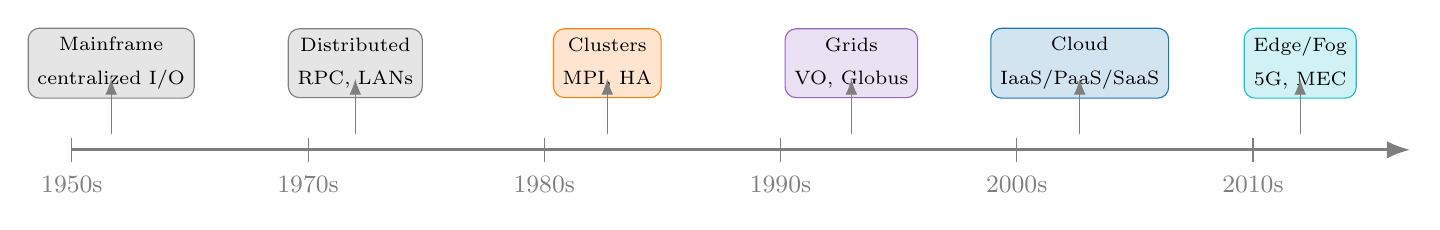
\begin{tikzpicture}[x=1cm,y=1cm]
    % timeline axis
    \draw[very thick,neutralgray,-{Latex[length=3mm]}] (0,0) -- (17,0);
    % ticks and labels
    \foreach \x/\year in {0/1950s,3/1970s,6/1980s,9/1990s,12/2000s,15/2010s}
      {\draw[neutralgray] (\x,0.15) -- (\x,-0.15) node[below,yshift=-2pt] {\small \year};}
    % nodes
    \node[fill=neutralgray!20,draw=neutralgray,rounded corners,align=center] (main) at (0.5,1.1) {\scriptsize Mainframe\\\scriptsize centralized I/O};
    \node[fill=neutralgray!20,draw=neutralgray,rounded corners,align=center] (dist) at (3.6,1.1) {\scriptsize Distributed\\\scriptsize RPC, LANs};
    \node[fill=orange!20,draw=orange,rounded corners,align=center] (cluster) at (6.8,1.1) {\scriptsize Clusters\\\scriptsize MPI, HA};
    \node[fill=fogpurple!20,draw=fogpurple,rounded corners,align=center] (grid) at (9.9,1.1) {\scriptsize Grids\\\scriptsize VO, Globus};
    \node[fill=cloudblue!20,draw=cloudblue,rounded corners,align=center] (cloud) at (12.8,1.1) {\scriptsize Cloud\\\scriptsize IaaS/PaaS/SaaS};
    \node[fill=edgeteal!20,draw=edgeteal,rounded corners,align=center] (edge) at (15.6,1.1) {\scriptsize Edge/Fog\\\scriptsize 5G, MEC};
    % connectors
    \draw[-{Latex[length=2mm]},neutralgray] (0.5,0.2) -- (0.5,0.9);
    \draw[-{Latex[length=2mm]},neutralgray] (3.6,0.2) -- (3.6,0.9);
    \draw[-{Latex[length=2mm]},neutralgray] (6.8,0.2) -- (6.8,0.9);
    \draw[-{Latex[length=2mm]},neutralgray] (9.9,0.2) -- (9.9,0.9);
    \draw[-{Latex[length=2mm]},neutralgray] (12.8,0.2) -- (12.8,0.9);
    \draw[-{Latex[length=2mm]},neutralgray] (15.6,0.2) -- (15.6,0.9);
  \end{tikzpicture}
  \caption{Computing paradigms evolution timeline from mainframes to edge/fog and cloud.}
  \label{fig:timeline}
\end{figure*}

Key definitions used in this survey follow authoritative sources: cloud computing as standardized by NIST~\cite{Mell2011NIST}; fog computing as the cloud extension toward the edge~\cite{Bonomi2012Fog,OpenFog2017RA,Chiang2016FogIoT}; mobile edge computing (MEC) per ETSI~\cite{ETSI2016MEC}; and edge computing as the broader decentralization of compute/storage to the periphery~\cite{Shi2016IoTJ,Satya2017Emergence}.

Concluding this section, the trend is toward a continuum where placement is fluid across devices, edge/fog, and cloud. This continuity motivates unified control, observability, and programming abstractions that hide heterogeneity while honoring locality and policy.

\section{Architectures}\label{sec:arch}
\subsection{Cloud-Only (Centralized) Architecture}
In cloud-only designs, applications and data are hosted in centralized data centers operated by cloud providers. Users access services over the Internet, leveraging virtualization and multi-tenancy to elastically scale~\cite{Armbrust2010CACM}. Fig.~\ref{fig:cloud} depicts the canonical pipeline from end-users through the Internet to virtualized compute, storage, and networking planes, with IaaS/PaaS/SaaS service layers.

\begin{figure}[t]
  \centering
  % Diagram 2: Cloud-Only Architecture
  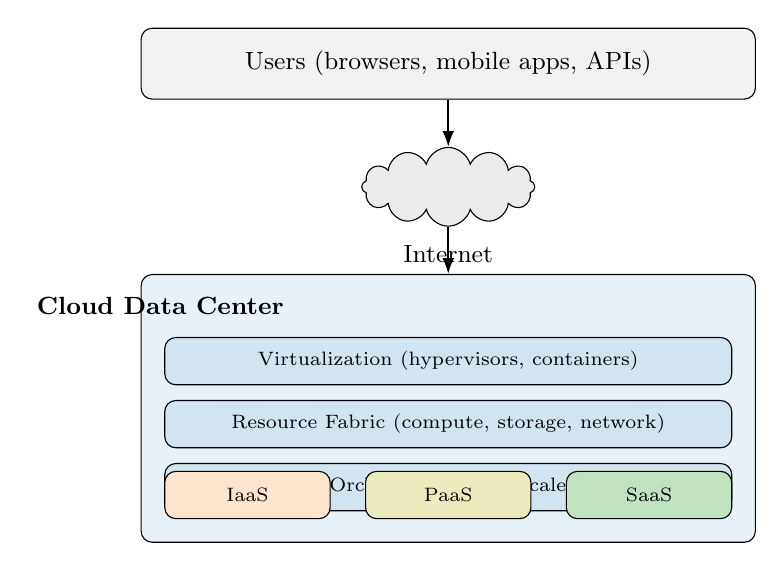
\begin{tikzpicture}[node distance=6mm]
    \node[draw,rounded corners,align=center,fill=neutralgray!10,minimum width=7.8cm,minimum height=0.9cm] (users) {\small Users (browsers, mobile apps, APIs)};
    \node[draw,cloud,cloud puffs=12,cloud ignores aspect,minimum width=2.2cm,minimum height=1.0cm,fill=neutralgray!15,below=of users] (internet) {};
    \node[below=1.2mm of internet] {\small Internet};
    \node[draw,rounded corners,fill=cloudblue!10,align=center,below=of internet,minimum width=7.8cm,minimum height=3.4cm] (dc) {};
    \node[align=left] at ($(dc.north west)+(0.25,-0.4)$) {\small \textbf{Cloud Data Center}};
    % virtualization layers
    \node[draw,rounded corners,fill=cloudblue!20,minimum width=7.2cm,minimum height=0.6cm,anchor=north west] at ($(dc.north west)+(0.3,-0.8)$) {\scriptsize Virtualization (hypervisors, containers)};
    \node[draw,rounded corners,fill=cloudblue!20,minimum width=7.2cm,minimum height=0.6cm,anchor=north west] at ($(dc.north west)+(0.3,-1.6)$) {\scriptsize Resource Fabric (compute, storage, network)};
    \node[draw,rounded corners,fill=cloudblue!20,minimum width=7.2cm,minimum height=0.6cm,anchor=north west] at ($(dc.north west)+(0.3,-2.4)$) {\scriptsize Management \& Orchestration (autoscale, multi-tenancy)};
    % service models
    \node[draw,rounded corners,fill=orange!20,minimum width=2.1cm,minimum height=0.6cm,anchor=south west] at ($(dc.south west)+(0.3,0.3)$) {\scriptsize IaaS};
    \node[draw,rounded corners,fill=gold!30,minimum width=2.1cm,minimum height=0.6cm,anchor=south] at ($(dc.south)+(0,0.3)$) {\scriptsize PaaS};
    \node[draw,rounded corners,fill=energygreen!30,minimum width=2.1cm,minimum height=0.6cm,anchor=south east] at ($(dc.south east)+(-0.3,0.3)$) {\scriptsize SaaS};
    % arrows
    \draw[-{Latex[length=2mm]},thick] (users) -- (internet);
    \draw[-{Latex[length=2mm]},thick] (internet) -- (dc);
  \end{tikzpicture}
  \caption{Cloud-only architecture: centralized data centers with virtualization and service models (IaaS/PaaS/SaaS).}
  \label{fig:cloud}
\end{figure}

\textit{Discussion and concluding note:} Cloud-only approaches maximize economies of scale and operational simplicity, but may violate latency and data residency constraints for time-critical workloads. They remain indispensable for global analytics and durable storage.

\subsection{Edge-Only (Decentralized) Architecture}
Edge-only designs shift computation, filtering, and short-term storage close to data sources (Fig.~\ref{fig:edgeonly}), minimizing wide-area traffic and enabling near-real-time actuation~\cite{Shi2016IoTJ,Satya2017Emergence}.

\begin{figure}[t]
  \centering
  % Diagram 3: Edge-Only Architecture
  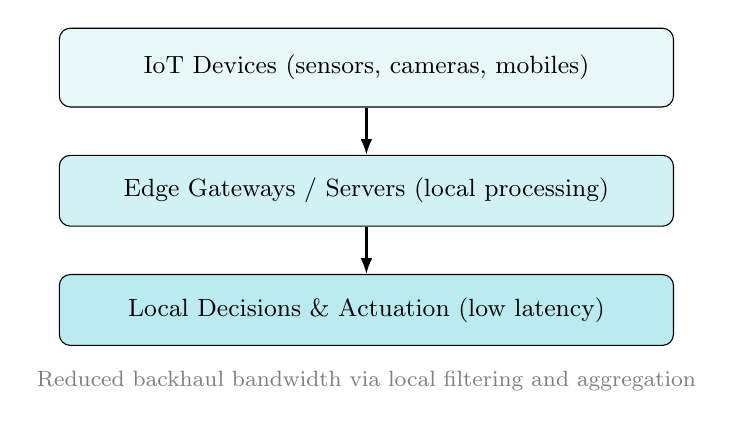
\begin{tikzpicture}[node distance=6mm]
    \node[draw,rounded corners,fill=edgeteal!10,align=center,minimum width=7.8cm,minimum height=1.0cm] (devices) {\small IoT Devices (sensors, cameras, mobiles)};
    \node[draw,rounded corners,fill=edgeteal!20,align=center,below=of devices,minimum width=7.8cm,minimum height=0.9cm] (gateway) {\small Edge Gateways / Servers (local processing)};
    \node[draw,rounded corners,fill=edgeteal!30,align=center,below=of gateway,minimum width=7.8cm,minimum height=0.9cm] (actions) {\small Local Decisions \& Actuation (low latency)};
    \draw[-{Latex[length=2mm]},thick] (devices) -- (gateway);
    \draw[-{Latex[length=2mm]},thick] (gateway) -- (actions);
    % bandwidth note
    \node[align=center,below=2mm of actions,neutralgray] {\footnotesize Reduced backhaul bandwidth via local filtering and aggregation};
  \end{tikzpicture}
  \caption{Edge-only architecture: decentralized processing near data sources for low-latency responses and bandwidth savings.}
  \label{fig:edgeonly}
\end{figure}

\textit{Discussion and concluding note:} Edge-only deployments excel for safety-critical control loops and privacy-preserving analytics but face constraints in aggregate compute capacity, manageability, and cross-edge coordination.

\subsection{Hybrid Cloud--Edge (Three-Tier) Architecture}
Most real systems adopt a hybrid model with device, edge/fog, and cloud layers (Fig.~\ref{fig:hybrid}). Time-critical tasks run near the edge; heavy compute, training, and global optimization are offloaded to the cloud. Intermediate fog nodes aggregate and coordinate among edges~\cite{Chiang2016FogIoT,ETSI2016MEC}.

\begin{figure}[t]
  \centering
  % Diagram 4: Hybrid Cloud-Edge Architecture
  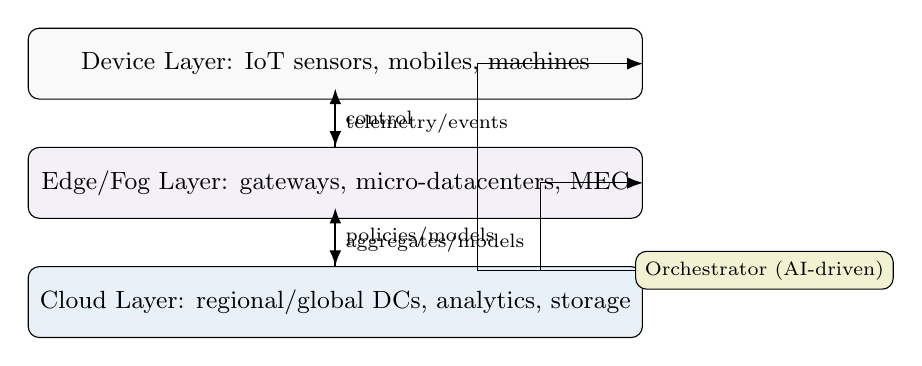
\begin{tikzpicture}[node distance=6mm]
    % Layers
    \node[draw,rounded corners,fill=neutralgray!05,align=center,minimum width=7.8cm,minimum height=0.9cm] (device) {\small Device Layer: IoT sensors, mobiles, machines};
    \node[draw,rounded corners,fill=fogpurple!10,align=center,below=of device,minimum width=7.8cm,minimum height=0.9cm] (edgefog) {\small Edge/Fog Layer: gateways, micro-datacenters, MEC};
    \node[draw,rounded corners,fill=cloudblue!10,align=center,below=of edgefog,minimum width=7.8cm,minimum height=0.9cm] (cloudl) {\small Cloud Layer: regional/global DCs, analytics, storage};
    % data flows
    \draw[-{Latex[length=2mm]},thick] (device) -- node[right]{\scriptsize telemetry/events} (edgefog);
    \draw[-{Latex[length=2mm]},thick] (edgefog) -- node[right]{\scriptsize aggregates/models} (cloudl);
    \draw[-{Latex[length=2mm]},thick] (cloudl) -- ++(-0,1.2) node[midway,right]{\scriptsize policies/models};
    \draw[-{Latex[length=2mm]},thick] (edgefog) -- ++(0,1.2) node[midway,right]{\scriptsize control};
    % orchestrator
    \node[draw,rounded corners,fill=gold!20,align=center,above right= -3mm and -1mm of cloudl] (orch) {\scriptsize Orchestrator (AI-driven)};
    \draw[-{Latex[length=2mm]},thin] (orch.west) -- ++(-1.2,0) |- (edgefog.east);
    \draw[-{Latex[length=2mm]},thin] (orch.west) -- ++(-2.0,0) |- (device.east);
  \end{tikzpicture}
  \caption{Hybrid three-tier architecture across device, edge/fog, and cloud layers with bi-directional data flows and AI-driven orchestration.}
  \label{fig:hybrid}
\end{figure}

\textit{Discussion and concluding note:} Hybrid architectures reconcile latency and scale while enabling progressive deployment. They necessitate robust placement, state synchronization, and policy enforcement across administrative domains.

\subsection{Comparative Analysis of Computing Models}
Fig.~\ref{fig:compare} summarizes cloud, fog, and edge trade-offs along latency, compute/storage capacity, cost, and typical use cases.

\begin{figure}[t]
  \centering
  % Diagram 5: Comparative Analysis as a table-like figure
  \renewcommand{\arraystretch}{1.2}
  \begin{tabular}{@{}p{1.8cm}p{1.2cm}p{1.6cm}p{1.5cm}p{2.4cm}@{}}
    \toprule
    \textbf{Model} & \textbf{Latency} & \textbf{Compute/Storage} & \textbf{Cost} & \textbf{Typical Use Cases} \\
    \midrule
    Cloud & High & Very High & Pay-as-you-go & Global analytics, training, batch processing \\
    Fog & Medium & Medium & Moderate & Aggregation, regional coordination, pre-processing \\
    Edge & Very Low & Low--Medium & Hardware-heavy & Real-time control, privacy-preserving inference \\
    \bottomrule
  \end{tabular}
  \caption{Comparative view of cloud, fog, and edge computing characteristics.}
  \label{fig:compare}
\end{figure}

\section{Challenges}\label{sec:challenges}
The cloud--edge continuum introduces interdependent challenges spanning systems, networking, and operations (Fig.~\ref{fig:mindmap}).

\begin{figure*}[t]
  \centering
  % Diagram 6: Key Challenges Mind Map
  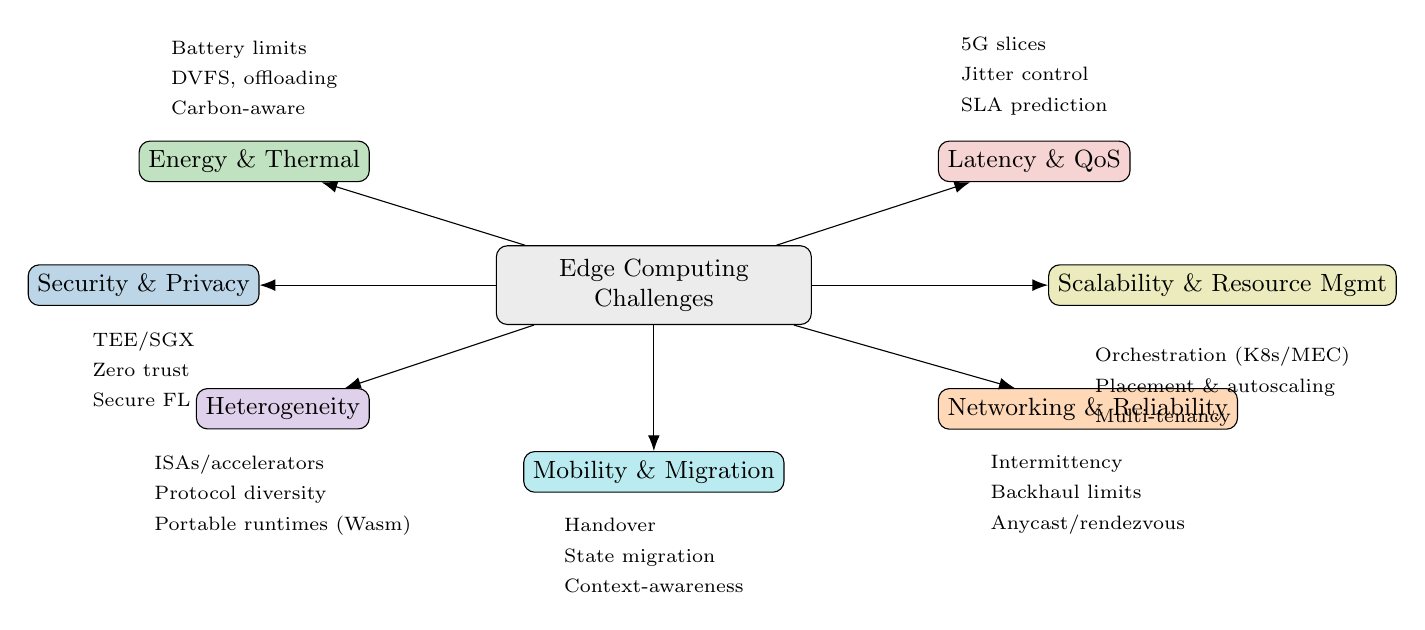
\begin{tikzpicture}[every node/.style={font=\small},node distance=8mm]
    \node[draw,rounded corners,fill=neutralgray!15,align=center,minimum width=4.0cm,minimum height=1.0cm] (center) {Edge Computing\\Challenges};
    % branches
    \node[draw,rounded corners,fill=gold!30,right=30mm of center] (scal) {Scalability \& Resource Mgmt};
    \node[draw,rounded corners,fill=latencyred!20,above right=8mm and 16mm of center] (qos) {Latency \& QoS};
    \node[draw,rounded corners,fill=orange!30,below right=8mm and 16mm of center] (net) {Networking \& Reliability};
    \node[draw,rounded corners,fill=energygreen!30,above left=8mm and 16mm of center] (energy) {Energy \& Thermal};
    \node[draw,rounded corners,fill=cloudblue!30,left=30mm of center] (sec) {Security \& Privacy};
    \node[draw,rounded corners,fill=fogpurple!30,below left=8mm and 16mm of center] (hetero) {Heterogeneity};
    \node[draw,rounded corners,fill=edgeteal!30,below=16mm of center] (mob) {Mobility \& Migration};
    % connectors
    \foreach \n in {scal,qos,net,energy,sec,hetero,mob} {\draw[-{Latex[length=2mm]}] (center) -- (\n);}    
    % sub-branches (examples)
    \node[below=4mm of scal,align=left] {\scriptsize Orchestration (K8s/MEC)\\\scriptsize Placement \& autoscaling\\\scriptsize Multi-tenancy};
    \node[above=2mm of qos,align=left] {\scriptsize 5G slices\\\scriptsize Jitter control\\\scriptsize SLA prediction};
    \node[below=2mm of net,align=left] {\scriptsize Intermittency\\\scriptsize Backhaul limits\\\scriptsize Anycast/rendezvous};
    \node[above=2mm of energy,align=left] {\scriptsize Battery limits\\\scriptsize DVFS, offloading\\\scriptsize Carbon-aware};
    \node[below=2mm of sec,align=left] {\scriptsize TEE/SGX\\\scriptsize Zero trust\\\scriptsize Secure FL};
    \node[below=2mm of hetero,align=left] {\scriptsize ISAs/accelerators\\\scriptsize Protocol diversity\\\scriptsize Portable runtimes (Wasm)};
    \node[below=2mm of mob,align=left] {\scriptsize Handover\\\scriptsize State migration\\\scriptsize Context-awareness};
  \end{tikzpicture}
  \caption{Mind map of key challenges for edge computing across systems, networking, and operations.}
  \label{fig:mindmap}
\end{figure*}

\subsection{Scalability and Resource Management}
Edge environments are resource-constrained and geographically distributed. Containers provide lightweight isolation compared to VMs, but orchestration at scale across heterogeneous sites remains immature relative to cloud counterparts~\cite{Mao2017MEC,Mach2017MEC}. Scheduling must jointly optimize latency, throughput, and energy under fluctuating demand and failures. Concluding, there is a need for intent-driven, hierarchy-aware orchestration that spans device/edge/fog/cloud with robust multi-tenancy.

\subsection{Networking, Connectivity, and Reliability}
Intermittent wireless links, variable backhaul, and diverse access technologies complicate consistent QoS. 5G/MEC reduce radio latency but end-to-end guarantees require placement-aware routing, congestion control, and service function chaining~\cite{ETSI2016MEC}. In conclusion, cross-layer co-design is essential to bridge application SLOs and network realities.

\subsection{Latency and Quality of Service}
Ultra-low-latency applications (e.g., industrial control, AR/VR) are sensitive to jitter and tail latency. Predictive models for QoS can guide proactive scaling and pre-warming of functions, particularly for serverless platforms. Concluding, robust percentile-tail management and SLA prediction are first-order design goals.

\subsection{Security and Privacy}
Decentralization enlarges the attack surface. Confidential computing (TEEs), remote attestation, encryption at rest/in transit, and zero-trust access are vital~\cite{Schuster2015VC3}. Privacy-preserving analytics (federated learning and secure aggregation) mitigate data exfiltration risks~\cite{McMahan2017FL,Bonawitz2017SA}. Concluding, verifiable trust and privacy budgets should be built into edge data pipelines.

\subsection{Heterogeneity}
Hardware diversity (CPUs, GPUs, TPUs, NPUs), instruction sets, and accelerators, alongside protocol variety, complicate portability. WebAssembly and container images for multiple architectures improve portability, but performance portability remains an open challenge~\cite{Haas2017Wasm}. Concluding, standardized execution substrates and interface descriptions are needed.

\subsection{Energy Efficiency and Sustainability}
Battery-powered devices and thermally constrained sites necessitate energy-aware computing (DVFS, adaptive offloading) and carbon-aware scheduling that shifts delay-tolerant workloads to greener regions/times~\cite{Liu2015GLB}. Concluding, sustainability should be a first-class objective across placement, networking, and model selection.

\subsection{Cost Optimization}
While edge reduces bandwidth costs via local processing, it introduces CAPEX (hardware) and OPEX (remote management). Transparent costing models and joint optimization of placement and data movement are required. Concluding, economics must be integrated with technical scheduling decisions.

\subsection{Mobility Support}
User and device mobility requires session continuity, stateful migration, and location-aware routing. Techniques such as predictive handover and micro-state replication can preserve QoE for vehicular and mobile AR use cases~\cite{Abbas2018Survey}. Concluding, mobility must be elevated to a first-class dimension in orchestration.

\section{Applications}\label{sec:applications}
\subsection{Smart Cities and Public Infrastructure}
City-scale sensing and actuation benefit from local inference (traffic signals, public safety) with cloud-based planning and policy optimization. Healthcare monitoring leverages wearables and home sensors for continuous telemetry and edge filtering, while cloud aggregates support population-level analytics.

\subsection{Autonomous Vehicles and Intelligent Transportation}
Autonomous systems rely on multi-modal sensing (LiDAR, radar, cameras) and near-sensor inference for safety. Edge sites at RSUs and road-side cabinets support collaborative perception; the cloud supports fleet-scale learning and map updates.

\subsection{AR/VR and Real-Time Media}
Interactive applications require motion-to-photon latency below human perceptual thresholds. Edge rendering and encoding coupled with cloud asset management deliver immersive experiences with constrained backhaul.

\subsection{Industry 4.0}
Industrial IoT uses digital twins, predictive maintenance, and closed-loop control. Edge gateways ensure deterministic response on the factory floor, while the cloud provides model training and supply-chain integration.

\subsection{Edge AI}
Deploying ML at the edge reduces latency and preserves privacy. Federated learning trains global models without centralizing raw data, complemented by secure aggregation and TEEs for confidentiality~\cite{McMahan2017FL,Bonawitz2017SA,Schuster2015VC3}. Concluding, model compression and hardware-aware NAS are crucial for sustainable edge AI.

\section{Future Directions}\label{sec:future}
\subsection{AI-Driven Orchestration}
Learning-based schedulers can predict demand, pre-warm functions, and optimize placement across the continuum in real time.

\subsection{Blockchain-Assisted Security}
Smart contracts for decentralized access control and audit can complement traditional PKI for IoT/edge trust, though performance and cost trade-offs remain open.

\subsection{Confidential Computing and Privacy}
TEEs and emerging confidential GPUs enable verifiable processing on untrusted sites; combining with differential privacy and federated methods can strengthen end-to-end confidentiality~\cite{Schuster2015VC3}.

\subsection{Serverless at the Edge}
Function-as-a-Service adapted for constrained nodes must mitigate cold starts, enable fine-grained autoscaling, and expose latency SLOs. Portable runtimes (e.g., Wasm) are promising substrates~\cite{Haas2017Wasm}.

\subsection{WebAssembly-Based Runtimes}
Wasm provides a secure, lightweight, and portable execution format suited for heterogeneous hardware, enabling language-agnostic deployment with near-native performance.

\subsection{6G and AI-Native Networks}
6G envisions AI-native control loops and integrated sensing/communications, amplifying the need for co-designed compute-network orchestration~\cite{Saad2019SixG}.

\subsection{Carbon-Aware Scheduling and Green Computing}
Shifting delay-tolerant compute to low-carbon regions and periods, model sparsification, and right-sizing resources can reduce environmental impact without sacrificing SLOs~\cite{Liu2015GLB}.

\subsection{Standardization and Interoperability}
Open interfaces across orchestration, telemetry, and security (attestation) are required to tame heterogeneity and promote portability across vendors and domains~\cite{ETSI2016MEC,OpenFog2017RA}.

\section{Conclusion}\label{sec:conclusion}
This review articulated the architectural foundations, systemic challenges, and application opportunities spanning the cloud--edge continuum. Cloud-only designs deliver scale, edge-only deployments deliver immediacy, and hybrid models reconcile both through layered placement and orchestration. Progress hinges on unifying abstractions, verifiable trust, AI-driven operations, and sustainability-aware optimization. With continued advances in 5G/6G, confidential computing, serverless runtimes, and federated learning, future systems can be both performant and privacy-preserving, efficient and sustainable.

\section*{Acknowledgment}
This work synthesizes publicly available research and standards. Author and affiliation placeholders should be replaced prior to submission.

\begin{thebibliography}{99}

\bibitem{Mell2011NIST}
P. Mell and T. Grance, ``The NIST Definition of Cloud Computing,'' NIST Special Publication 800-145, 2011.

\bibitem{Armbrust2010CACM}
M. Armbrust \emph{et al.}, ``A View of Cloud Computing,'' \emph{Communications of the ACM}, vol. 53, no. 4, pp. 50--58, 2010.

\bibitem{Shi2016IoTJ}
W. Shi, J. Cao, Q. Zhang, Y. Li, and L. Xu, ``Edge Computing: Vision and Challenges,'' \emph{IEEE Internet of Things Journal}, vol. 3, no. 5, pp. 637--646, 2016.

\bibitem{Satya2017Emergence}
M. Satyanarayanan, ``The Emergence of Edge Computing,'' \emph{Computer}, vol. 50, no. 1, pp. 30--39, 2017.

\bibitem{Mao2017MEC}
Y. Mao, C. You, J. Zhang, K. Huang, and K. B. Letaief, ``A Survey on Mobile Edge Computing: The Communication Perspective,'' \emph{IEEE Communications Surveys \& Tutorials}, vol. 19, no. 4, pp. 2322--2358, 2017.

\bibitem{Mach2017MEC}
P. Mach and Z. Becvar, ``Mobile Edge Computing: A Survey on Architecture and Computation Offloading,'' \emph{IEEE Communications Surveys \& Tutorials}, vol. 19, no. 3, pp. 1628--1656, 2017.

\bibitem{Varghese2018NextGen}
B. Varghese and R. Buyya, ``Next Generation Cloud Computing: New Trends and Research Directions,'' \emph{Future Generation Computer Systems}, vol. 79, pp. 849--861, 2018.

\bibitem{Bonomi2012Fog}
F. Bonomi, R. Milito, J. Zhu, and S. Addepalli, ``Fog Computing and Its Role in the Internet of Things,'' in \emph{Proc. MCC}, 2012, pp. 13--16.

\bibitem{OpenFog2017RA}
OpenFog Consortium Architecture Working Group, ``OpenFog Reference Architecture for Fog Computing,'' 2017.

\bibitem{Chiang2016FogIoT}
M. Chiang and T. Zhang, ``Fog and IoT: An Overview of Research Opportunities,'' \emph{IEEE Internet of Things Journal}, vol. 3, no. 6, pp. 854--864, 2016.

\bibitem{ETSI2016MEC}
ETSI, ``Mobile Edge Computing (MEC); Framework and Reference Architecture,'' ETSI GS MEC 003 V1.1.1, 2016.

\bibitem{Satya2009Cloudlets}
M. Satyanarayanan, P. Bahl, R. Caceres, and N. Davies, ``The Case for VM-Based Cloudlets in Mobile Computing,'' \emph{IEEE Pervasive Computing}, vol. 8, no. 4, pp. 14--23, 2009.

\bibitem{Yousefpour2019FogSurvey}
A. Yousefpour \emph{et al.}, ``All One Needs to Know About Fog Computing and Related Edge Computing Paradigms,'' \emph{Journal of Systems Architecture}, vol. 98, pp. 289--330, 2019.

\bibitem{Deng2020EdgeIntelligence}
S. Deng, H. Zhao, W. Fang, J. Yin, S. Dustdar, and A. Y. Zomaya, ``Edge Intelligence: The Confluence of Edge Computing and Artificial Intelligence,'' \emph{IEEE Internet of Things Journal}, vol. 7, no. 8, pp. 7457--7469, 2020.

\bibitem{McMahan2017FL}
H. B. McMahan, E. Moore, D. Ramage, S. Hampson, and B. A. y Arcas, ``Communication-Efficient Learning of Deep Networks from Decentralized Data,'' in \emph{Proc. AISTATS}, 2017.

\bibitem{Schuster2015VC3}
F. Schuster \emph{et al.}, ``VC3: Trustworthy Data Analytics in the Cloud Using SGX,'' in \emph{Proc. IEEE S\&P}, 2015, pp. 38--54.

\bibitem{Haas2017Wasm}
A. Haas \emph{et al.}, ``Bringing the Web up to Speed with WebAssembly,'' in \emph{Proc. PLDI}, 2017, pp. 185--200.

\bibitem{Liu2015GLB}
Z. Liu, M. Lin, A. Wierman, S. Low, and L. L. H. Andrew, ``Geographical Load Balancing with Renewables,'' \emph{IEEE/ACM Transactions on Networking}, vol. 23, no. 6, pp. 1954--1967, 2015.

\bibitem{Saad2019SixG}
W. Saad, M. Bennis, and M. Chen, ``A Vision of 6G Wireless Systems: Applications, Trends, Technologies, and Open Research Problems,'' \emph{IEEE Network}, vol. 34, no. 3, pp. 134--142, 2020.

\bibitem{Abbas2018Survey}
N. Abbas, Y. Zhang, A. Taherkordi, and T. Skeie, ``Mobile Edge Computing: A Survey,'' \emph{IEEE Internet of Things Journal}, vol. 5, no. 1, pp. 450--465, 2018.

\bibitem{Bonawitz2017SA}
K. Bonawitz \emph{et al.}, ``Practical Secure Aggregation for Privacy-Preserving Machine Learning,'' in \emph{Proc. ACM CCS}, 2017, pp. 1175--1191.

\end{thebibliography}

\end{document}

